\documentclass[12pt]{article}
\usepackage{nouvellesCommandes}
\usepackage{cedric}
\usepackage{fourier}
\DeclareMathAlphabet{\mathcal}{OMS}{cmsy}{m}{n}
\setlength\parindent{0pt}
\title
{
  \faireTitre[p=.50,h=5]{Amplificateurs de probabilités}
}

%\lhead{}
%\rhead{T\up{ale} \textsc{Es} 1, lycée St-Ex}
\begin{document}

\maketitle
\thispagestyle{fancy}

Pour un sport à deux joueurs, on étudie deux règles de départage les deux opposants $A$ et $B$.

On suppose que : \quad
\begin{enligneItemize}
  \item le jeu se dispute par manches indépendantes les unes des autres.
  \item chacune est remportée
    par l'un
    avec probabilités :
    \begin{tabular}[t]{rcc}
      vainqueur   & $A$ & $B$ \\
      probabilité & $p$ & $q$ \\
      \multicolumn{3}{r}{\hint{avec $p+q = 1$}}
    \end{tabular}
\end{enligneItemize}

\moinsLigne[4]
%\vspace{-3\baselineskip}
\section{Un score fixé à atteindre}
\subsection{Cas général}
D'abord, on déclare victorieux le premier joueur à avoir remporté $k \in \N^{*}$ manches \guillemets{en tout}.

\begin{enumerate}
  \item
    À partir de combien de manches jouées
    est-on sûr de pouvoir départager les deux joueurs ?
    %Au maximum,
    %avant de pouvoir départager les deux joueurs,
    %combien de manches faudra
\end{enumerate}
%On suppose d'abord que les joueurs jouent \hint{jusqu'à} trois manches,

On suppose que les joueurs décident de jouer ces $2k-1$ parties de toutes façons.

\hfiller\hint{quitte à ce que les dernières manches n'aient aucune chance de changer le résultat du match}

Le nombre de sets remportés par le joueur $A$ est modélisé par la variable aléatoire $N$.

\begin{enumerate}[resume]
  \item Montrer que $N$ suit la loi binomiale $\B(m,r)$ pour deux paramètres $m, r$ à préciser.
  \item Rappeler : \quad
    \begin{enligneItemize}
      \item les valeurs possibles $N(\Omega)$ et les probabilités associées
      \item l'espérance $\E[N]$ et la variance $\Var(N)$.
    \end{enligneItemize}
\end{enumerate}
\moinsLigne[2.5]
\subsection{Cas général}
On choisit maintenant $k=2$ : il faut remporter deux manches en tout pour remporter le match.
\begin{enumerate}[resume]
  \item
    \begin{enumerate}
      \item Expliciter alors la loi binomiale $\B(m,r)$ suivie.
      \item En déduire la probabilité $f_{1}(p)=\P(N \ge 2)$.

        On montrera l'expression : \quad $f_1(p) = 3 \cdot p^2 - 2\cdot p^3$.
    \end{enumerate}
  \item \label{fUn}Montrer les propriétés : \quad
    \begin{minipage}[t]{6cm}
        \begin{itemize}
            \item $\forall p \ge \frac{1}{2}, \quad f_1(p) \ge p$,
            \item $f_1\big(\frac{1}{2}\big) = \frac{1}{2}$,
        \end{itemize}
      \end{minipage}
    \begin{minipage}[t]{7cm}
        \begin{itemize}
            \item $\forall p \in \intervalleoo{0}{1}, \quad f_1(1-p) = 1-f(p)$,
            \item $f_1$ croissante.
        \end{itemize}
      \end{minipage}
    %\begin{objetGauche} %{{{
    %  \begin{minipage}{10cm}
    %    \begin{multicols}{2}
    %      \begin{itemize}
    %        \item $\forall p \ge \frac{1}{2}, \quad f_1(p) \ge p$,
    %        \item $f_1\big(\frac{1}{2}\big) = \frac{1}{2}$,
    %        \item $\forall p \in \intervalleoo{0}{1}, \quad f_1(1-p) = 1-f(p)$,
    %        \item $f_1$ croissante.
    %      \end{itemize}
    %    \end{multicols}
    %  \end{minipage}
    %  \finObjet
    %  Montrer les propriétés : \quad
    %\end{objetGauche}
    %\begin{enligneItemize}
    %  \item $\forall p \ge \frac{1}{2}, \quad f_1(p) \ge p$,
    %  \item $f_1\big(\frac{1}{2}\big) = \frac{1}{2}$,
    %  \item $\forall p \in \intervalleoo{0}{1}, \quad f_1(1-p) = 1-f(p)$,
    %  \item $f_1$ croissante.
    %\end{enligneItemize}
      %}}}
\end{enumerate}

\subsection{Simulation avec Scilab}
\begin{imageGauche}{majorite.pdf}[][-\baselineskip][width=75mm]
  \lstinputlisting{binomAffich.sce}
\end{imageGauche}
\begin{enumerate}[resume]
  \item Commenter les lignes \scilab{2} et \scilab{6} : quelles sont les valeurs prises par \scilab{p} dans la boucle \scilab{for} ?
    \begin{enumerate}
      \item À quelles valeurs de \scilab{k} correspondent les courbes obtenues ?
      \item À quelle valeur de \scilab{k} la courbe formée d'un segment correspond-elle ?
      \item Quel profil de courbe obtiendrait-on si on prenait une valeur élevée pour \scilab{k} ?
    \end{enumerate}
\end{enumerate}

\section{Deux manches d'affilée}
On nomme maintenant vainqueur le premier à gagner deux manches successivement \hint{\guillemets{d'affilée}}.

On considère donc l'événement : \quad
\raz
\begin{tabular}[t]{r@{}l}
  $D_A$ & ${}={}$\guillemets{le joueur $A$ remporte le match}                    \\
        & ${}={}$\guillemets{$A$ est le premier à gagner deux manches d'affilée} \\
\end{tabular}


\subsection{Conditionnement par le premier tirage}
Dans cette partie, on suppose que le premier set a été remporté par le joueur $A$. \hint{soit l'événement $A_1$}

On calcule la probabilité conditionnelle : \quad $\P_{A_1}(D_A)$

\begin{enumerate}[resume]
  \item
    \begin{objetGauche}
      \begin{varwidth}[t]{10cm}
        \begin{description}
          \item [Sequence 1] $AA$
          \item [Sequence 2] $ABB$
          \item [Sequence 3] $ABAA$
          \item [Sequence 4] $ABABB$
        \end{description}
      \end{varwidth}
      \finObjet
      Pour chacune des séquences ci-contre, donner le gagnant
    \item On note $T$ le rang d'apparition de la première répétition.
      \begin{enumerate}
        \item Pour chacune des séquences, donner la valeur de $T$.
        \item À quelle condition sur $T$ le joueur $A$ remporte-t-il la partie ?
      \end{enumerate}
    \end{objetGauche}
    \vspace{-3\baselineskip}

    \begin{objetGauche}[-.5\baselineskip]
      $
      \begin{array}[t]{rccc}
        \toprule
        k=             & 2 & 4    & 6      \\
        \midrule
        \P_{A_1}(T=k)= & p & qp^2 & qpqp^2 \\
        \bottomrule
      \end{array}
      $
      \finObjet
      \begin{enumerate}[resume]
          \setcounter{enumii}{2}
        \item Justifier les probabilités ci-contre :

          Proposer, en fonction de l'entier $n\ge 1$, l'expression de la probabilité : \quad $\P_{A_1}(T=2n)$.
      \end{enumerate}
    \end{objetGauche}
    \moinsLigne
  \item
    \begin{enumerate}
      \item Montrer la convergence et donner la somme de la série \quad $S = 1 + pq + (pq)^2 + (pq)^3 + \ldots$
      \item En déduire que : \quad $\P_{A_1}(D_{A}) = \frac{p}{1-pq}$.
    \end{enumerate}
\end{enumerate}
\moinsLigne
\subsection{Conclusion}
\begin{enumerate}[resume]
  \item
    \begin{enumerate}
      \item Justifier : \quad $\P_{B_1}(D_{A}) = 1-\frac{q}{1-pq}$.
      \item Par la formule des probabilités totales, en déduire : \quad $\P(D_{A}) = \frac{(1+q)\cdot p^2}{1-pq}$.
    \end{enumerate}
  \item Vérifier, pour $f_2(p) = \P(D_{A})$, les quatre hypothèses de la question \ref{fUn}
\end{enumerate}

\section{Un certain nombre de jeux d'avance}
Soit $n \ge 1$ un entier fixé.

On déclare maintenant victorieux le premier joueur à avoir une avance de $n$ manches remportées.
\subsection{Modélisation}

On note $a_i$ la probabilité \hint{conditionnelle !} que le joueur $A$ remporte le match \hint{arrive à $n$ manches d'avance} lorsqu'il a $i$ points d'avance. \quad \hint{\ldots sachant que\ldots}

\begin{example}[Plus précisément]~\\
  Soit $X_k$ \hint{\resp $Y_k$} le score, $k$ manches après le début du match, en nombre de manches, de $A$ \hint{\resp $B$}.

  Alors pour n'importe quelle valeur de $k \in \N$ avant la fin du match, on a : \quad $a_i = \P_{[X_k=Y_k+i]}(A \text{ gagne le match})$
\end{example}

\begin{enumerate}[resume]
  \item Justifier : \quad 
    \begin{enligneItemize}
      \item $a_{n}=1$ et $a_{-n}=0$,
      \item $a_{0}$ est la probabilité absolue que le joueur $A$ remporte le match.
    \end{enligneItemize}
    \moinsLigne
  \item
    Par la formule des probabilités totales lorsque le score est $i$, montrer : \quad $a_{i} = p \cdot a_{i+1} + q \cdot a_{i-1}$.
\end{enumerate}
\subsection{Résolution}
\begin{enumerate}[resume]
  \item \label{geometrique}Vérifier que l'on peut écrire
    $p \cdot (a_{i+1} - a_i)
    =
    q \cdot (a_{i} - a_{i-1})$.

    En déduire que les $(a_{i} - a_{i-1})_{i\in\entiers{-n+1}{n}}$ forment une progression géométrique.
  \item
    \begin{enumerate}
      \item Par sommation télescopique, justifier : \quad
        \smash
        {%
          %$\sum_{\mathclap{i=-n+1}}^{n}(a_{i} - a_{i-1}) = a_{n} - a_{-n}$.
          $\sum_{\mathclap{i=k}}^{\ell}(a_{i} - a_{i-1}) = a_{\ell} - a_{k-1}$.
        }%
      \item \label{telescopique}En déduire que : \quad
        \begin{enligneItemize}
          \item \quad $\sum_{\mathclap{i=-n+1}}^{n}(a_{i} - a_{i-1}) = 1$,
          \item \quad $\sum_{\mathclap{i=-n+1}}^{0}(a_{i} - a_{i-1}) = a_0$.
        \end{enligneItemize}
        \moinsLigne[2]
    \end{enumerate}
  \item Grâce aux questions\ref{geometrique} et\ref{telescopique}, montrer : \quad
    $a_{-n+1} \cdot
    \frac
    {%
      1-
      \big(\frac{q}{p}\big)^{2n\!\!}
    }%
    {%
      1-\frac{q}{p}
    }%
    =1
    $.
    %$a_0 \cdot
    %\frac
    %{%
    %  \big(\frac{q}{p}\big)^{n+1} -
    %  \big(\frac{q}{p}\big)^{-n+1}
    %}%
    %{%
    %  1-\frac{q}{p}
    %}%
    %=1
    %$.
  \item En déduire que : \quad $a_0 =
    \frac
    {%
      1-
      \big(\frac{q}{p}\big)^{n}
    }%
    {%
      1-
      \big(\frac{q}{p}\big)^{2n\!\!}
    }%
    $ \quad  puis montrer : \quad
    $a_0 = p^{n} \cdot \frac{q^{n} - p^{n}}{q^{2n} - p^{2n}}$.
  \item 
    \begin{enumerate}
      \item Simplifier l'expression de $a_0$ pour $n=1$ et pour $n=2$.
      \item Que se passe-t-il si $q=p=\frac{1}{2}$ ?
    \end{enumerate}
\end{enumerate}
  
\section{Comparaison des trois approches}

\begin{objetGauche}
  \begin{minipage}[t]{7cm}
    \lstinputlisting[linerange= debAff-finAff]{comparaisonAffichage.sce}
    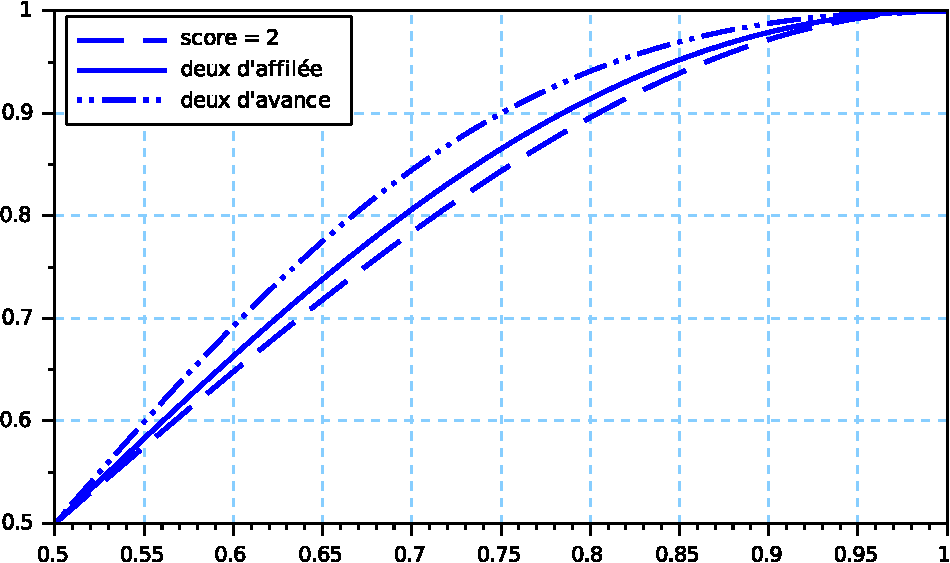
\includegraphics[width=\linewidth]{comparaisonDesTroisGrille.pdf}
  \end{minipage}
  \finObjet
  \lstinputlisting[linerange= debFon-finFon]{comparaisonAffichage.sce}
\end{objetGauche}
\begin{enumerate}[resume]
  \item Compléter \hint{ligne \scilab{8}} la fonction \scilab{deux_d_affilee} selon le modèle des deux autres.
  \item Si le joueur $A$ a 3 chances sur $4$ de gagner chaque manche, quelle est la probabilité qu'il gagne le match, sous la modalité \guillemets{deux d'affilée} ?
  \item Quelle méthode parmi les trois illustrées semble le mieux départager les joueurs ?
  \item Quel est l'\hint{énorme !} avantage \important{pratique} de la méthode \guillemets{score fixé à atteindre} sur les deux autres ?
\end{enumerate}

\end{document}
